\chapter{Collaborative Filtering\index{Collaborative Filtering}}


\textsf{ In this chapter we explain Collaborative Filtering in more detail,
along with giving details of the NETFLIX prize and the lead up to present work.
We explain about the data and the approach to the solution of the problem.}


\section{Recommender Systems\index{Recommender Systems}}
Internet technologies have greatly become a part of our lives, there are many
occasions when we need help in taking certain decisions. Recommendations in
general is ubiquitous when there is a need to make choices without sufficient
personal experience, we rely on feedback from users on certain products, we make
use of recommendation letters for jobs, reviews of movies and books
\cite{Resnick:1997:RS:245108.245121}. Consider for a movie streaming company
like NETFLIX, where people can watch movies from a huge collection, have been
collecting the ratings of the movies from the users. This data can be considered
as our \emph{training data}, it is explicitly obtained from the users. Using
this training data the company makes predicitions of movies the users are likely
to prefer watching more than others. This is only one of the different types of
recommender systems. 
\subsection{Recommender System Strategies}
The strategies for building recommender systems are based on the type of data
available and how the data is used. On a broad sense the two main approaches are
\emph{content-based filtering}, in which the items are characterized based on 
certain attributes, and recommendation are made based on filtering similar
items. In the second approach, \emph{collaborative filtering}, the ratings
previously given by users is used to build a model, which is then used to make
predictions. The term Collaborative Filtering was first termed by Tapestry
\cite{Goldberg:1992:UCF:138859.138867}, which was one of the first recommender
systems. Recommender
Systems produce possibly accurate prediction of relationship between elements of
different classes based on previous knowledge or the \emph{training data}. This
training data could be explicitly obtained in the form of ratings given by
users or it could be implicit knowledge(purchase
history, browsing history, search patterns,mouse movements etc), which can be
used when explicit knowledge is insufficient \cite{Hu:2008:CFI:1510528.1511352}.
But however in this thesis work we model our system based on explicit
knowledge. 

Modern recommender systems are based on the collaborative filtering, which again
is of two types, the \emph{nearest neighbor approach} and the \emph{latent
factor approach}. In the nearest neighbor methods, items or users are given
certain attributes which decides the proximity between them. Further this sense
of proximity is used predict an item for an user. The second approach is
the latent factor approach, which characterizes the users and the items together
in building the model. Matrix factorization is used to build these models, likes
of SVD is very useful. \emph{Rating matrix} proves to be important, as it
charectarizes both items and users as its vectors. 

\subsection{The Problem Formulation}
Our problem could be defined as a matrix completion problem, where the matrix is
formed by placing the users $u$ along the rows and the movies $m$ along the
rows. The entries in this matrix are filled through the \emph{training data},
which is collection of $n$ \emph{quadruples}, with the format
(\emph{user(k)},\emph{movie(k)},\emph{rating(k)},\emph{timestamp(k)}), where
$k=1,2...,n$. The $1 \leq user \leq u$ and $1 \leq movie \leq m$ are the
range of the users and the movies, where as the ratings, $1<rating<5$. The
\emph{Rating
matrix} is defined as $R\in\mathbb{R}^{u,m}$, \\
\begin{equation}
  R[i,j]=\begin{cases}
    rating(k), & \text{$i=user(k), j=movie(k)$}.\\
    ?, & \text{otherwise}.
  \end{cases}
\end{equation}

where \emph{'?'} are the cases where the \emph{user-movie} relation is unknown.
These are the values which needs to be predicted. Once the \emph{'?'} values are
computed, recommendations could be made depending on the required tolerance
level, \emph{user-movie} pairs with predicted ratings higer than the tolerant
value(threshold) can be selected for making recommendations. Hence this problem
can be viewed as a \emph{matrix completion} problem. In this thesis work, we
will compute the unknowns for a certain subset called the \emph{test set}. \\

Let us denote the completed matrix, or rather the reconstructed matrix	 by
\emph{$\hat_{R}$}. We intend to obtain the
\emph{$\hat_{R}$}, by reproducing it through a simple product of two matrices
with reduced \emph{inner dimension}. Let $P\in\mathbb{R}^{u,f}$ and
$Q\in\mathbb{R}^{f,m}$ are the two matrices with reduced inner dimension
\emph{f}. 


Let us through a very simple example see the principle behind collaborative
filtering.

 \begin{example}
   We show 4 users who have rated 4 movies, we tabulate the preferences, in the
form of ratings on the scale of 1 to 5,  as shown below. The users are along the
rows and items along the columns, rating  given by \textit{user i} to
\textit{item j} is the real valued entry (i,j) in  the rating matrix.  \\

\begin{tabular}{c|cccc}
       & Titanic & Braveheart & The Lion King & Dreamcatcher  \\
\hline
John   & 5 & 5 & 2 & -   \\
Dave   & 2 & - & 3 & -   \\
Alice  & - & 5 & - & 3   \\
Bob    & 3 & - & - & 5   \\
\end{tabular}

From the above, we can consider the rating matrix to be \\

$R_{i,j}$ =
$ \begin{pmatrix}
  5 & 5 & 2 & ? \\
  2 & ? & 3 & 5 \\
  ? & 5 & ? & 3  \\
  3 & ? & ? & 5
 \end{pmatrix} $\\
 
 Using matrix factorization, we simply do a SVD on $R$ to get, $U$ and $V$,
which denote the user space and the movie space. \\
 
 $U$ =
 $\begin{pmatrix}
  1.12 & 1.49 & 0.48  \\
  1.31 & -0.52 & 0.59  \\
  1.13 & 0.67 & -0.52  \\
  1.39 & 0.05 & 0.45 
 \end{pmatrix} $
 \hspace*{10mm}
 $V$ =
 $\begin{pmatrix}
  1.12 & 1.49 & 0.48  \\
  1.31 & -0.52 & 0.59  \\
  1.13 & 0.67 & -0.52  \\
  1.39 & 0.05 & 0.45 
 \end{pmatrix} $\\

 Once we have factored the rating matrix $R$, we can get the missing values by
approximating the sparse rating matrix into a full one,  $\hat{R}=U*V'$ \\

$\hat{R}_{i,j}$ =
 $\begin{pmatrix}
  4.78 & 4.98 & 1.97 & 3.61 \\
  1.98 & 1.97 & 2.85 & 4.81 \\
  2.75 & 4.71 & 1.40 & 2.94  \\
  2.94 & 3.32 & 2.75 & 4.79
 \end{pmatrix} $\\
 
 With this approximation, we can make predictions of ratings of movies which the
users have not seen. 
 
\end{example}

\section{NETFLIX}
Entertainment has been one of the most significant integral part of human
society and has evloved along with modern technologies. In todays internet
driven society, IPTV(Internet Protocol Television) is gaining popularity in
delivering television and cinema content to viewers. IPTV mainly consists of
three groups, \\
\begin{enumerate}%for small alpha-characters within brackets.
\item Live Television - Live telecast or transmission to the viewers with only
the transmission delay, example live news show.
\item Time-shifted Television which is also called as catch-up TV, in which the
viewers can watch the content which is stored and available at any point of
time. 
\item Video on Demand - here the viewers are given a wide range of TV shows and
movies to choose. They can watch anything they wish, the content is streamed to
the viewers computer which the user can pause and watch later. NETFLIX provides
its content throught this method. \\
This owes to a great extent to the success of NETFLIX, since through on Demand
system NETFLIX is able to cater to individual tastes of users. NETFLIX can
collect statistics pertaining to individual users' choices and the most
important metric is the \emph{ratings}. NETFLIX aims to greatly improve the
customer satisfaction and retention by providing a greatly personalised
experience to the users. The importance of personalization is such, that NETFLIX
ignited the research attempts in the Mathematical and Computer Science soceity
to develop methods which could do predictions for movie likeability quotient.
Such attempts have certainly been fruitful to NETFLIX as is evident from the
fact that as of today 33 million members view over 1 billion hours of TV shows
and movies through NETFLIX per month.
\end{enumerate}

\subsection{NETFLIX Prize}
During October 2006, NETFLIX challenged the research community to beat the
performance in terms of accuracy of their own recommendation system
\emph{Cinematch} by 10\%. The NETFLIX prize challenge was provided with over 100
million ratings from around half a million users and 18 thousand movies. This
data was collected during the period october 1998 and December 2005. The
challenge would take place over a period of three years, and a progress prize of
50 thousand USD would be awarded each year to the team which would produce the
best improvements. Finally at the end of three years a Grand Prize of 1 Million
USD would be given to the team with the best results in terms of RMSE. Their
benchmark system \emph{Cinematch}, based on \emph{Pearson correlation} which is
straightforward statistical linear model produces an RMSE of 0.9525 on test
data. Hence to qualify to win the Grand Prize which accounts for 10\%
improvement over \emph{Cinematch}, which corresponds to RMSE of 0.8563 on
\emph{quiz set}. On an event of a tie the time of entry would be taken into
account, and this is exactly what happened on 26 July 2009, team BellKor's
Pragmatic Chaos won the challenge by margin of 20 minutes. Table 2.1 shows the
performance of top 12 teams, \cite{NETFLIX_Prize:Online}
\begin{table}
\centering 
\begin{tabular}{|c|c|c|c|} \hline %\hline
%-------------------------------------------------------------------
$Rank$ & $Team$ & 
$RMSE$ &  $Percent Improvement$  \\ 
\hline
%-------------------------------------------------------------------
$ 1$
& $BellKor's Pragmatic Chaos$
& $0.8567$
& $10.06$ \\ %\hline
%-------------------------------------------------------------------
$ 2$
& $The Ensemble$
& $0.8567$
& $10.06$ \\ %\hline
%-------------------------------------------------------------------
$ 3$
& $Grand Prize Team$
& $0.8582$
& $9.90$\\  %\hline
%-------------------------------------------------------------------
$ 4$
& $Opera Solutions and Vandelay United$
& $0.8588$
& $9.84$\\  %\hline
%-------------------------------------------------------------------
$ 5$
& $Vandelay Industries !$
& $0.8591$
& $9.81$ \\%\hline
%-------------------------------------------------------------------
$ 6$
& $PragmaticTheory$
& $0.8594$
& $9.77$ \\ %\hline
%-------------------------------------------------------------------
$ 7$
& $BellKor in BigChaos$
& $0.8601$
& $9.70$ \\ %\hline
%-------------------------------------------------------------------
$ 8$
& $Dace$
& $0.8612$
& $9.59$ \\ %\hline
%-------------------------------------------------------------------
$ 9$
& $Feeds2$
& $0.8622$
& $9.48$  \\%\hline
%-------------------------------------------------------------------
$ 10$
& $BigChaos$
& $0.8623$
& $9.47$ \\ %\hline
%-------------------------------------------------------------------
$ 11$
& $Opera Solutions$
& $0.8623$
& $9.47$ \\ %\hline
%-------------------------------------------------------------------
$ 12$ 
& $BellKor$        
& $0.8624$ 
& $9.46$  \\ \hline 
\end{tabular}
\caption{RMSE of Top 12 Teams}
\label{tab:TopTeams}
\end{table}
-
\subsection{The NETFLIX dataset}
NETFLIX had been collecting data since October 1998,
as of June 2007 the company had collected over 1.9 billion ratings from more
than 11.7 million subscribers over 85 thousand titles \refname{The NETFLIX
Prize}. The company then recieved over 2 million ratings per day. To provide
data for the competition the company did two seperate random sampling processes,
the first one to obtain th eentire Prize dataset and second for the qualifying
and probe set. The condition for selecting the users was that they should have
given minimum of 20 ratings. \\

 Basically the company has seggregated the data based on time, the latest data
form the Test Data and the initial data form the training data. The
\emph{Training data} includes the \emph{Probe set} which is meant for fine
tuning before submissions. The training data is basically a text file consisting
of triplets entries like, (UserID, MovieID, Rating). There are 100 million such
entries which form the training set. The training set also included the probe
set consisting of 1,408,395 triplets, this could be used by the competitors to
fine tune their algorithms before submission. NETFLIX also collected the latest
ratings of all the users in the training set to form the \emph{Qualifying set}.
This set was in the form (UserID,MovieID,DatrofRating), where the ratings were
known only to the judjes. The qualifying set was again divided into 2 groups,
the \emph{Quiz set} and \emph{Test set}. The quiz set having 1,408,342 ratings
was used to update the Leaderboard, the RMSE on this quiz set was released to
the competitors. The test set having 1,408,789 ratings was only used by the jury
to adjudge the winner. \cite{Bennett07thenetflix}\\



 
\begin{table}
\begin{center}
    \begin{tabular}{|ccc|}
        \hline
         TRAINING SET  & ~ &  Probe set  \\ 
         100480507 & ~ & 1408395   \\ \hline       
    \end{tabular} \\
    \caption[]{Training Data}
     \begin{tabular}{|c|c|}
       \hline
       Test Set  & Quiz Set  \\ 
       1408789 & 1408342 \\ \hline       
    \end{tabular}
    \caption{Qualifying Data}     
\end{center}
\end{table}


\section{Matrix Factorization for Collaborative Filtering}
With Collaborative Filtering it involves filtering for information through
collaboration among interacting groups, for example users and movies. Matrix
factorization happens to be the first choice for collaborative filtering, as
matrices can hold high dimensional information in tabular form, and can be
factored into products of smaller matrices. \emph{In matrix factorization the
users and items are mapped onto a joint latent factor space of reduced dimension
$f$, and the inner product of the user vector with item vector gives the
corresponding interaction.} \cite{Koren:2009:MFT:1608565.1608614}
\subsection{Basic Matrix Factorization}
Matrix factorization is mainly about a more compact representation of the large
training data which is obtained by dimensionality reduction.
\cite{Liu:2010:GLA:1821715.1821722}. 
\emph{We want to quantify the nature or the characteristics of the movies
defined by a certain number of aspects (factors), i.e we are trying to
generalize the information (independent and unrelated ratings matrix) in a
concise and descriptive way.} \cite{citeulike:4563139} All the movies can be
described by certain features like overall rating, cast, wether its an action
flick or romantic drama, how did it fare during the first week of it release
etc. Similarly a user can also be described based on the same factors, wether
the user is liberal in rating or very critical, does the user have certain
favourite cast, if the user prefers action over romance, does the user watch and
rate movies on the first week of its release etc. What we have here is a common
factor space in which we tend to generalize the relationships between the users
and movies, based on these factors. Hence the 8.5 billion ratings can be
explained in lot fewer factors. We are generalizing the independent individual
unrelated ratings to a more concise and descriptive form. Here what we have done
is through meaningful generalities, concised the data, the reverse also holds
good, i.e by concising the data or in other words by reducing the dimension, we
can generalize the description of the large data. The Singular Value
Decomposition exactly helps in achieving this. This is explained crudely with an
example,\\

\begin{example}
Let us say we have around ten aspects which are used to describe movies and
users. Each movie has ten numerical values, which exemplifies the ten aspects.
Similarly the users also have ten such values. We can combine these values to
obtaing a single rating value for each user-movie pair, bu multiplying the
corresponding terms and summing them up. Let us consider a movie Die Hard whose
aspects might be something like, action=1.2, chickflick=-1, and so on. Let us
consider a user Joe whose aspects are, action=3, and chickflick=-1. So the
overall rating for the movie Die Hard given by Joe is, $3*1.2+-1*-1+..$ =
$(3.6+1+..)$. It clearly shows that Joe would evetually like the movie Die
Hard, which is evident from the high rating value obtained.   
\end{example}\\

 The model in its most basic form is built around the following \\
 $R=P*Q'$
 where $P\in\mathbb{R}^{u,f}$ and $Q\in\mathbb{R}^{i,f}$. The number $f$ is
decided by trial and error, higher the value better the predictions, however
beyond certain value it will not contribute to the accuracy significantly. This
value decides the number of \emph{factors} which will be used to characterize
users and movies. This is analogous to dimension reduction. \\
The individual vector in $P$, $p_{u}\in\mathbb{R}^f$ represents an user, it
gives a measure of the qualities represented by the $f$ factors. Similarly,
every item is represented by a $q_{i}\in\mathbb{R}^f$ which says about the $f$
qualities pertaining to the items, i.e movies. We cannot for sure say what are
the qualities which these factors represent. The task of predicting a rating
for a user $u$ gives for a movie $i$, can be computed as an inner product, \\

$\hat{r}_{ui}=q_{i}^Tp_{u}.$ \\

This dot product gives the iteraction between the item $i$ and the user $u$. The
challenge is in the mapping of all the users and items to a joint latent factor
space of dimensionality $f$ \cite{Koren:2009:MFT:1608565.1608614}.\\
Singular Value Decomposition (SVD), would be first choice for such a
factorization, as it helps a great deal in identifying the the best top-most
factors, i.e by selecting the left and right singular vectors corresponding to
top $n$ singular values. \\

\subsection{Dimension Reduction}
Matrix factorization and dimension-reduction go hand-in-hand, the dimension of
our rating matrix is very high and along with factorizing the matrix it is
important to reduce the dimensions of the factored matrices. It is the inherent
property of SVD that we can decide the rank or the number of \emph{factors} we
need in order to get the best approximation of our User-Movie rating model. By
dimension reduction we get to express the information which was initially
presented
in a matrix of dimension 480189x17770 having around 85 billion ratings in much
smaller space with only \emph{k} factors, where \emph{k} is the reduced
dimension.
While a reduction in dimension, also aids in removal of noise, however too low
dimension
can result in removal of useful information as well. Hence it is important to
decide on an optimal dimension. Through an example below we can further justify
the
need for dimension reduction,
\begin{example}
 Consider movies like "Harry Potter", "Chronicles of Narnia", "Lord of the
Rings" etc, there are very large number of movies similar to this. By saying
similar what we mean is that these movies all have certain common factors, like
they all are fantasy movies, they all are novel based movies. Hence instead of
retaining all these movies, we can replace them with certain latent factors,
which are much fewer than the number of items or movies, and hence the dimension
is reduced.
\end{example}


\subsection{Different Models}
Collaborative Filtering based Recommender Systems are built using either
Neighbourhood-methods or model-based methods
\cite{Koren:2008:FMN:1401890.1401944}. Our approach involves the
model-based method, which has proved to be one of the most effective approach as
is evident from the NETFLIX Challenge and large number of research articles on
the same topic. To have a good Recommender System, it is important to achieve
good accuracy and also to keep the model simple. Keeping this in mind, we try to
build a model which accounts for significant predictor variables, like the
temporal dynamics, user-bias, movie-bias etc. However we initially analyze these
individual predictors and after careful analyses, we blend them together in the
final model to achieve the best RMSE. The main principle behind our model of
laten factor modelling, supplemented with the removal of biases pertaining to
users, movies and temporal variations. Below table shows the various models we
use, 

\begin{table}
\centering 
\begin{tabular}{|c|c|} \hline %\hline
%-------------------------------------------------------------------
$Model No.$ & $Model$   \\ 
\hline
%-------------------------------------------------------------------
$ 1$
& Naive Models based on user/movie means  \\ %\hline
%-------------------------------------------------------------------
$ 2$
& Bias-Model\\ %\hline
%-------------------------------------------------------------------
$ 3$
& Temporal model - SVD  \\ %\hline
%-------------------------------------------------------------------
$ 4$
& Temporal model - ALS  \\ \hline
%------------------------------------------------------------------- 
\end{tabular}
\caption{Different models}
\label{tab:Models}
\end{table}


\subsubsection{Data Representation}
Before beginning discussion on the models, we show a detailed representation of
the training and the test data which are used in this work, which are in the
form of matrices, i.e, the rating matrix $R$, the date matrix $D$,
these comprise the training data. The test data is in the form of three
matrices, probe set $P_{probe}$, test set $Q_{test}$, quiz set
$Q_{quiz}$ and finally $Q_{all}$ which consists of the entire test
data. Each of the above matrices except $D$ are in the form,  \\
$\mathcal{R} = \{r_{ij} \exists \mbox{ in } R \mid \mbox{user } i \in
\mathcal{U} \mbox{ have rated movie } j \in \mathcal{M} \}$, \\
where $r_{ij}$ is the rating for the corresponding user-movie pair and is also
the $(i,j)^{th}$ entry in their respective matrices. The matrix $D$ however
has the same structure of $R$, but with the date of rating instead of the
rating itself.

\subsubsection{Basic Naive model} We start by doing some rating predictions
based on the average of all the ratings in the $R$ matrix, which is 3.5769. We
simply use this value for any unknown user-movie combination. Moving ahead we
could use the \emph{user-mean}, to calculate the unknown rating, for example if
we need a prediction for user $u$, for any of the movies we simply use the
average of all the ratings given by user $u$. Similarly to predict the unknown
rating for some movie $i$, we could simply use the average rating of that movie
over all the known ratings given to that movie in the matrix $R$.  
\subsubsection{Bias model} Moving ahead we try out new models which takes care
of the inherent biases of various kinds in the data. Bias model removes the
anomalies, if any in the data. Biases in this cintext can be considered to be
variations in the ratings which are caused by certain effects associated with
the users or movies, independetly of the interaction between the two groups.
The interaction is captured in the factorization part and the inner products of
the interacting vectors. The main purpose of doing this is, by separating the
interaction and the biases will help us in subjecting only the interaction
portion of the data which is more critical
\cite{Koren:2010:CFT:1721654.1721677}.
The $Baseline predictors$ capture these biases which do not involve user-movie
interaction. While factorization these biases are removed only to be added after
factorization, i.e, post-processing. 
\subsubsection{Temporal Bias + SVD model} The main objective in this thesis is
to capture the temporal dynamics within the data and include them into the
$baseline predictors$ through two major temporal effects, each involving users
and movies. However in this thesis the temporal effects related only to movies
is considered. We have considered the movie-bias to be a function of time, which
can capture the changes in popularity of movies in course of time, owing to
number of external triggering factors like the actor in the movie winning a
major award. Also the users tend to drift with their rating styles with time,
for example a liberal user might for some reason become a more critical in
rating movies. \\
 This model uses the good old Singular Value Decomposition for the factorizing
the rating matrix. But however it is evident that owing to the sparsity in the
data SVD proves to be not very effective. To avoid this imputation can be
employed but this can be very expensive in terms of memory. 
\subsubsection{Temporal Bias + ALS model} Owing to the disadvantage of the SVD
as will be explained in future chapters, we employ an alternative method in
Alternating Least Squares. It is an iterative method with initial guessed
values for $M$ and alternatively solving for $U$ and $M$ until convergence. This
method is computationally demanding but can be parallelized easily. If $R$ is
the rating matrix, we formulate a low-rank matrix approximation problem as shown
below,
\begin{equation}
 (U,M)=arg \min_{U,M} \mathcal{L}^{\emph{emp}}(R,U,M)
\end{equation}
where $U$ and $M$ $\in \mathbb{R}$ and have $n_f$ columns. The symbolic
representation of the problem is shown below,


The $x^s$ denote the known ratings in the matrix $R$ and $\in \emph{I}$, where
\emph{I} is the known ratings set and $n$ is the number of known ratings in
total. In general the problem is of the type, 
\begin{equation}
 \|{Ax-b}\|
 \label{eq:OLS}
\end{equation}
\begin{equation}
 \|{R-UM^T}\|
 \label{eq:ALS}
\end{equation}
where we are trying to minimize the above in Frobenius norm, which is matrix
equivalent of 2-norm. We wish to solve the above problem in a least squares
sense, but since it is not in the form of ordinary least squares(OLS). We try to
convert the type shown in Equation ~\ref{eq:ALS} to the type shown in Equation
~\ref{eq:OLS}.
\begin{figure}[h!]
\includegraphics[width=1\textwidth]{ALS_FIG.pdf}

\caption{ALS Decomposition}
\label{fig:ALS Decomposition}
\end{figure}


Let us consider the first row of $R$, which will have all the ratings
given by the fist user. Let us assume the user has seen movies 1, 213, 315,
1744, 2133, 7044, 9012, 12344 and 16890  so in a total of 9 movies. Forming a
vector of the known ratings for the first user we have $\begin{bmatrix}
                                          1 & 213 & 315 & 1744 & 2133 & 7044 &
9012 & 12344 & 16890                                    
                                          \end{bmatrix}
$, let
this be denoted by $b$. We initialize the $M$ matrix in a particular way, and as
shown in the Figure 2.1 it has $n_m$ rows and $n_f$ columns. The matrix $U$ has
$n_u$ rows and $n_f$ columns. For the case of the first user we can form a
sub-matrix of $M$, denote this by $M_u$. This matrix $M_u$ will have all the
rows from $M$ corresponding to the movies seen by the user $u$, the first user
in this case. Let $\boldmath{u}$ be the row vector from $U$ corresponding to the
considered user, .i.e, first user. Now we have three components $R(1,:)$, the
row vector having the nine ratings of the nine movies seen by user 1, $u_1$ the
unknown first row of $U$ matrix, $M_u$, a submatrix of $M$ consisting of the
rows corresponding to the movies rated by the user 1. Figure 2.2 shows the
symbolic representation of this single ordinary least squares problem
formulation, $ \|{M_uu-R(1,:)}\|$. This is done for all the users to obtain the
$U$ matrix. Next this $U$ matrix is used to estimate the new $M$ matrix. The $U$
and $M$ are estimated alternatively until some convergence criteria is
satisfied. 


\begin{figure}[h!]

\includegraphics[width=0.6\textwidth]{ALS_FIG2.pdf}
\caption{OLS }
\label{fig:OLS Decomposition}
\end{figure}









